\documentclass{uc3mpracticas}

\usepackage{helvet}
\usepackage{caption}
\usepackage{listings}
\renewcommand{\familydefault}{\sfdefault}


%%%%%%%%%%%%%%%%%%%%%%%%%%%%%%%%%%%%%%%%%%%%%%%%%%%%%%%%%%%%%%%%%%%%%%%%%%%%%%%%
%%%                   Plantilla Prácticas UC3M                               %%%
%%%                Universidad Carlos III de Madrid                          %%%
%%%                   Alejandro Valverde Mahou                               %%%
%%%%%%%%%%%%%%%%%%%%%%%%%%%%%%%%%%%%%%%%%%%%%%%%%%%%%%%%%%%%%%%%%%%%%%%%%%%%%%%%

%Permitir cabeceras y pie de páginas personalizados
\pagestyle{fancy}

%Path por defecto de las imágenes
\graphicspath{ {./images/} }

%Declarar formato de encabezado y pie de página de las páginas del documento
\fancypagestyle{doc}{
  %Cabecera
  \headerpr[1]{Sistemas de Producción}{}{Ingeniería del Conocimiento}
  %Pie de Página
  \footerpr{}{\textbf{UC3M}}{{\thepage} de \pageref{LastPage}}
}

%Declarar formato de encabezado y pie del título e indice
\fancypagestyle{titu}{%
  %Cabecera
  \headerpr{}{}{}
  %Pie de Página
  \footerpr{}{}{}
}


\appto\frontmatter{\pagestyle{titu}}
\appto\mainmatter{\pagestyle{doc}}


\begin{document}
  %Comienzo formato título
  \frontmatter


  %Portada 1 (Centrado todo)
  \centeredtitle{Images/LogoUC3M.png}{Grado en Ingeniería Informática}{Curso 2020/2021}{Ingeniería del Conocimiento}{Práctica 1: Sistemas de Producción}

  \vspace{55mm}

  \authors{Alba Reinders Sánchez}{100383444}{Alejandro Valverde Mahou}{100383383}{}{}{Grupo 83}{Leganés}

  \newpage

  %Índice
  \tableofcontents

  \newpage

  %Comienzo formato documento general
  \mainmatter

  \section{Introducción}

En esta primera práctica se aborda la implementación de un \textbf{sistema de producción} (\textit{SP}) en CLIPS que lleve a cabo la ejecución de una sesión de un especialista con un paciente en la que interactúan un humano y un robot \textit{NAO}, donde este último adopta el papel de especialista.

\begin{figure}[!h]
  \centering
  \includegraphics[width=.25\linewidth]{Images/nao.png}
  \caption*{Robot \textit{NAO}}
\end{figure}


En concreto, se crea un \textit{SP} con toda la información respecto a los personajes y el entorno en el que se lleva a cabo la interacción, así como posibles desviaciones durante la sesión en las que el robot debe reaccionar y modificar sus acciones en consecuencia.

\vspace{2mm}

La interacción entre el paciente y el robot se realiza a través del desarrollo de 2 juegos: el \textbf{Twister} y el \textbf{Tres en raya}. Además, el sistema está adecuado para tratar con pacientes que puedan presentar 2 personalidades distintas, aparte del comportamiento base, \textbf{despistado} y \textbf{enérgico}.

\vspace{2mm}

Se han elegido estos juegos por ser ejemplos de actividades sencillas, que requieren de un número reducido de reglas, para demostrar las aplicaciones de los \textit{SP}. Por el mismo motivo, se han elegido únicamente 2 posibles comportamientos básicos. Si se deseara aplicar sobre un problema real no serían suficientes, y sería necesario tener en cuenta un mayor número de personalidades.


\begin{figure}[!h]
  \centering
  \begin{minipage}{.52\textwidth}
    \centering
    
\includegraphics[width=.5\linewidth]{Images/3enraya.png}
    \caption*{Juego del Tres en Raya}
  \end{minipage}%
  \begin{minipage}{.52\textwidth}
    \centering
    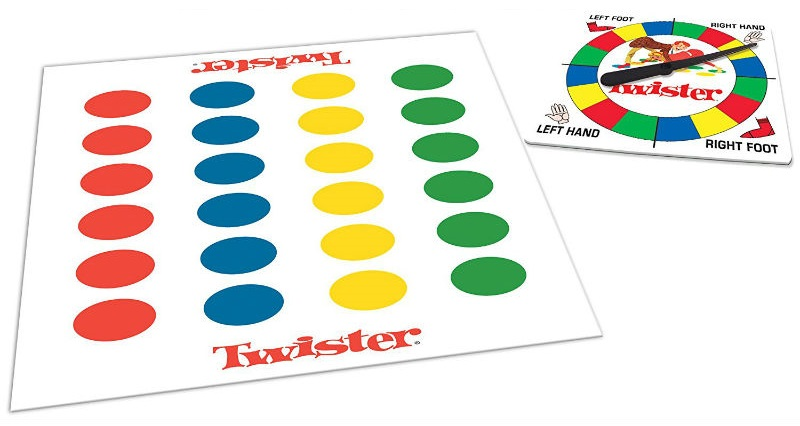
\includegraphics[width=.8\linewidth]{Images/twister.jpg}
    \caption*{Juego del Twister}
  \end{minipage}
\end{figure}

El documento consiste en el manual técnico con la descripción de la implementación, el manual de usuario con la explicación de cómo usar el programa, las pruebas realizadas y el análisis de los resultados, y para finalizar una serie de conclusiones y comentarios personales.


  \newpage

  \section{Manual técnico}

  El \textit{SP} está compuesto por la \textbf{ontología} y las \textbf{reglas}. A continuación, se explican ambas justificando todas las decisiones que se han tomado durante la implementación.

  \vspace{2mm}

  Los flujos de acciones que se han planteado para resolver los problemas son los siguientes, donde los estados de color rojo solo se pueden realizar si el \textit{paciente} es \textit{enérgico} y los de color verde si el \textit{paciente} es \textit{despistado}.


  \vspace{2mm}

  El flujo de una sesión consiste en: saludar al \textit{paciente} y explicarle el juego. Si se comprueba que el \textit{paciente} no lo ha entendido correctamente, se repite la explicación. Una vez el \textit{paciente} lo ha entendido, se procede a ejecutar el juego. Cuando finaliza el mismo, se comprueba si el \textit{paciente} tiene energías para seguir jugando. Si es así, se repite el juego. En caso contrario, se termina la sesión.

  \begin{figure}[!h]
    \centering
    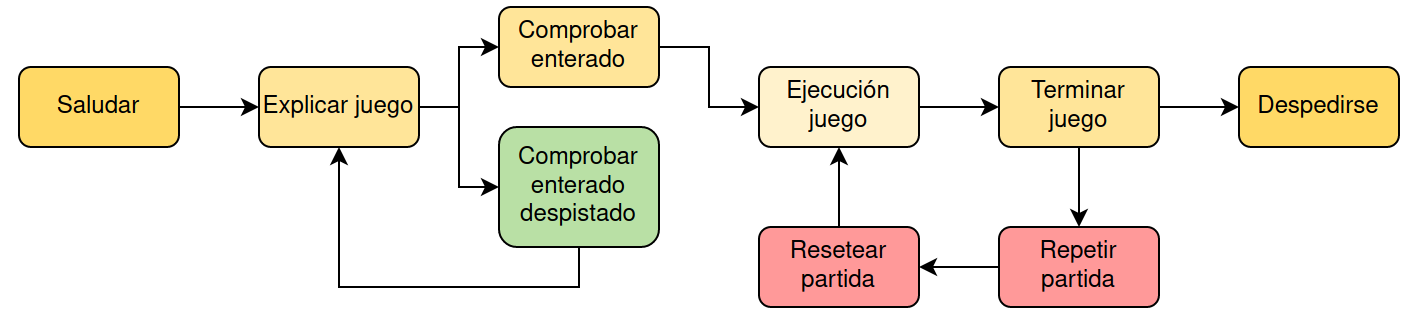
\includegraphics[width=.85\linewidth]{Images/flujo1.png}
    \caption*{Flujo genérico de una sesión}
  \end{figure}

  Si el juego elegido es el \textbf{Twister}, el flujo consiste en, una vez explicado y entendido el juego, seleccionar un color y extremidad que el \textit{paciente} tendrá que realizar. Si el \textit{paciente} la realiza correctamente, se pasará a elegir otro color y extremidad. Una vez se haga correctamente 5 veces, el juego terminará. Por otro lado, si el \textit{paciente} se cae, el juego terminará también.

  \vspace{2mm}

  Además, si el \textit{paciente} está despistado, se le repetirá el último comando y, en caso de que se lo tenga que repetir más de 6 veces, se considera que el \textit{paciente} está demasiado despistado para continuar y se termina la sesión. Por último, si el \textit{paciente} cambia su posición, se le repetirá todas las órdenes, para que pueda volver a colocarse correctamente.

  \begin{figure}[!h]
    \centering
    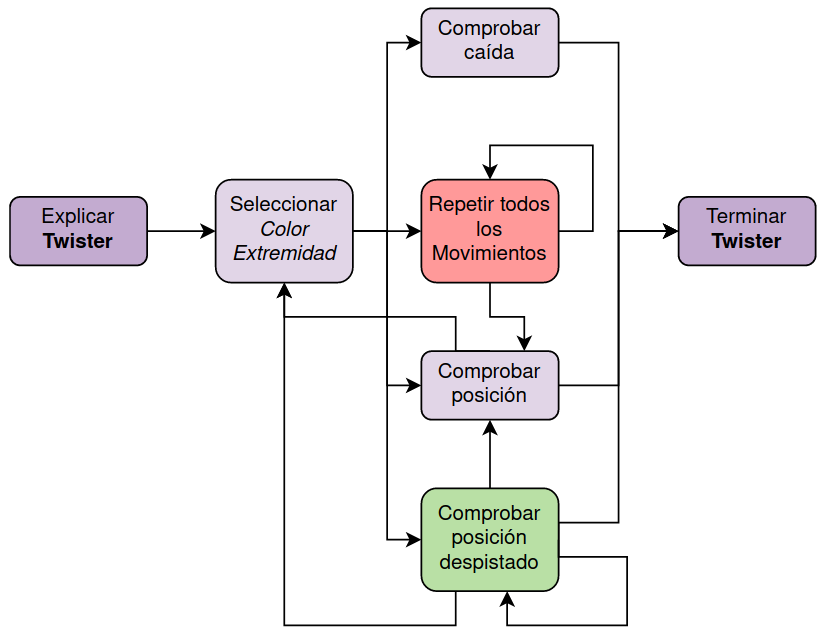
\includegraphics[width=.6\linewidth]{Images/flujo2.png}
    \caption*{Flujo del Twister}
  \end{figure}

  \newpage

  Si el juego es el \textbf{Tres en Raya}, el flujo consiste en, una vez explicado y entendido el juego, simular colocar una ficha por turnos, pasando del \textit{paciente} al \textit{robot} (empieza siempre el \textit{paciente}). Si el \textit{paciente} está despistado y no coloca ficha se le recuerda un máximo de 3 veces seguidas, y en caso de que siga despistado, se terminará la sesión. Por otro lado, si se despista un total de 6 veces, la sesión terminará, por el mismo motivo.

  \vspace{2mm}

  Si por el contrario tiene muchas energías y coloca ficha cuando no es su turno, se le regaña, y se le impedirá colocar la ficha. Además, si intenta colocar ficha fuera de turno más de 3 veces, se terminará la partida, y se le dará la victoria al \textit{robot}. Siempre que no haya tres en raya o un empate (todas las casillas ocupadas sin tres en raya) se seguirá el flujo del juego.

  \begin{figure}[!h]
    \centering
    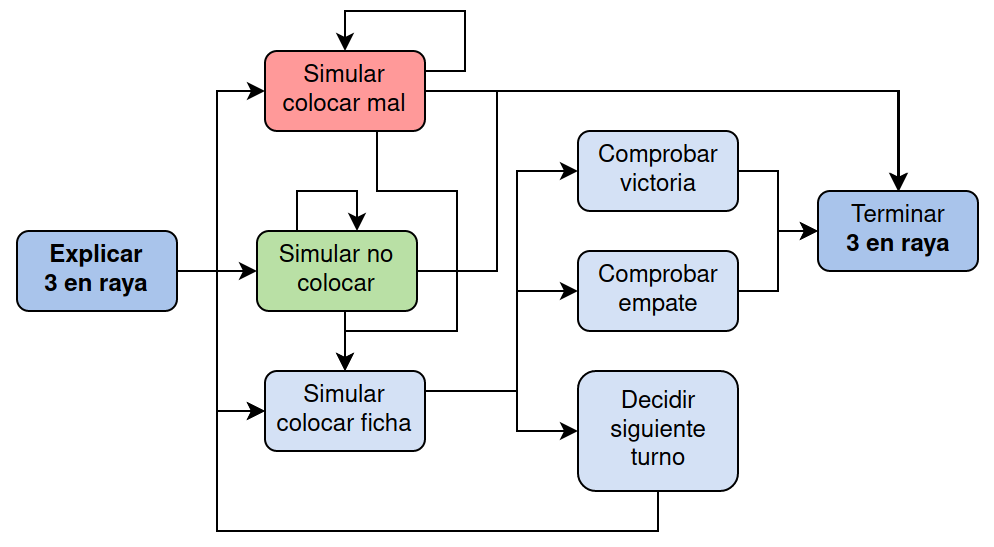
\includegraphics[width=.65\linewidth]{Images/flujo3.png}
    \caption*{Flujo del Tres en Raya}
  \end{figure}


  \subsection{Ontología}

  La ontología que se plantea para la solución está compuesta de las siguientes clases.

  \begin{itemize}
    \item \textbf{JUEGO} $\rightarrow$ Representa el juego que se va a llevar a cabo a lo largo de la sesión. Contiene, además del nombre (\textit{id}) del juego, la explicación del mismo, junto con la indicación de quién debe empezar (\textit{paciente} o \textit{robot}). Esto se ha decidido porque para cada juego comienza uno de los dos:

    \vspace{1mm}

    En el caso del \textbf{\textit{Twister}}, el \textit{robot} será siempre el que empiece la partida, dado que será el \textit{paciente} el que siempre 'juegue', mientras que el \textit{robot} elige las acciones.

    \vspace{2mm}

    Por otro lado, se ha decidido que para el caso del \textit{\textbf{Tres en Raya}} siempre empiece el paciente. Esto se ha hecho porque, en este juego, el jugador que comienza tiene ventaja y, dado que el juego forma parte de una terapia, se quiere potenciar que el \textit{paciente} gane con mayor probabilidad.

    \item \textbf{CONTROL} $\rightarrow$ Esta clase tendrá una única instancia, y se usa para localizar las distintas operaciones que controlan el sistema en una sola instancia. En el caso excepcional de que se repita la partida (comportamiento que solo puede darse con \textit{pacientes} de personalidad \textit{enérgica}) esta instancia se borra y se reinicia.

    \vspace{2mm}

    Esta clase permite controlar de quién es el turno, el número de ciclos, junto al número máximo de ciclos, el número de fallos, el juego que se lleva a cabo en la sesión, y el número de veces que se repite la partida.

    \item \textbf{PACIENTE} $\rightarrow$ Representa al paciente que está en la sesión. Se ha decidido usar una clase en lugar de un \textit{fact} para representarlo porque, además de la peronalidad del paciente, también almacena el nombre del mismo. Esto se hace para poder enviar mensajes personalizados, y que el paciente se encuentre en un ambienta más cómodo e informal.
    \item \textbf{COLOR} $\rightarrow$ Representa cada uno de los cuatro colores posibles para el juego del \textbf{\textit{Twister}}. Puede ser \textit{rojo}, \textit{verde}, \textit{amarillo} o \textit{azul}.

    \item \textbf{EXTREMIDAD} $\rightarrow$ Representa cada una de las cuatro extremidades posibles para el juego del \textbf{\textit{Twister}}. Puede ser \textit{pie derecho}, \textit{pie izquierdo}, \textit{mano derecha} o \textit{mano izquierda}.

    \item \textbf{ELECCION} $\rightarrow$ Representa cada una de las elecciones o comandos que hace el \textit{robot} y que tiene que realizar el \textit{paciente} en el juego del \textbf{\textit{Twister}}. Además del color y la extremidad elegidas, para poder realizar comprobaciones adicionales, se incluye el número de veces que se ha tenido que repetir una misma elección, y el orden por el que se han dicho.

    \item \textbf{CASILLA} $\rightarrow$ Representa cada una de las 9 casillas del juego del \textit{\textbf{Tres en Raya}}. Además de sus coordenadas, se tiene su valor, que puede ser \textit{vacío} si no se ha colocado nada todavía, o \textit{paciente} o \textit{robot}, en función de quién coloque la ficha.
  \end{itemize}



  \subsection{Reglas}

  Según se ha planteado el \textit{SP}, en la reglas reside toda la funcionalidad del sistema. Por ello, el número de reglas creadas es bastante grande. Sin embargo, considerando todas las distintas variaciones e interacciones que se han tenido en cuenta, resulta lógico que se necesiten más reglas.

  \vspace{1mm}

  Esta cantidad de reglas permite que los datos que se tienen que introducir por un usuario del sistema sea mínima, y hace que todo el flujo sea controlado por las reglas.

  \vspace{2mm}

  También destacar que, como se ha enfocado a dos personalidades concretas, hay reglas que son exclusivas para estas personalidades. Esto hace que al estar enfocado a una solución muy concreta, la resolución es mucho más detallada y potente. Pero a cambio se pierde capacidad de generalización a la hora de añadir nuevas personalidades.

  \vspace{1mm}

  Si se quisiera añadir un pesonalidad nueva habría que reescribir y modificar reglas, así como crear nuevas. A pesar de esto, se ha decidido esta forma para poder realizar un desarrollo de la sesión lo más completa posible.

  \subsubsection{Reglas genéricas}

  Estas reglas son las que sirven para ambos juegos y donde da igual la personalidad del paciente:

  \begin{itemize}
    \item \textbf{\textit{Saludar}}: el \textit{robot} saluda de manera personalizada al \textit{paciente} por su nombre.
    \item \textbf{\textit{Explicar}}: el \textit{robot} explica al \textit{paciente} el juego que se haya elegido.
    \item \textbf{\textit{Comprobar-enterado}}: el \textit{robot} comprueba que el \textit{paciente} se haya enterado de la explicación del juego.
    \item \textbf{\textit{Despedirse}}: el \textit{robot} se despide de manera personalizada del \textit{paciente} por su nombre.
  \end{itemize}

  Si el \textit{paciente} tiene de personalidad \textit{despistado}, existe la regla \textbf{\textit{Comprobar-enterado-despistado}} para repetir la explicación del juego y la regla \textbf{\textit{Demasiadas-equivocaciones-despistado}} para terminar la sesión porque se ha equivocado más de 6 veces y por tanto se considera que el \textit{paciente} puede no estar muy atento para continuar con el juego.

  \vspace{3mm}

  Se añade la regla \textbf{\textit{Repetir-partida}} para volver a jugar otra partida. Esto sucede exclusivamente si el \textit{paciente} es \textit{enérgico}, ya que se considera que puede que tenga más energías para seguir jugando.

  \vspace{1mm}

  Por lo tanto, una vez que se acaba una partida se activa esta regla y, dependiendo del juego, las siguientes: \textbf{\textit{Resetear-partida-tres-en-raya}} y \textbf{\textit{Resetear-partida-twister}}. Estas sirven para reiniciar las variables del juego.

  \vspace{2mm}

  Además, se crea la regla \textbf{\textit{Auxiliar-fin-reseteo}}, que lo que hace es finalizar el proceso de reinicio de variables.

  \vspace{2mm}

  Por último, se tiene la regla \textbf{\textit{Demasiadas-equivocaciones-energico}}, la cual tiene como fin terminar la sesión si el \textit{paciente} intenta colocar un ficha cuando no es su turno más de 3 veces. Este comportamiento es exclusivo del \textit{enérgico}, ya que se considera que ha hecho demasiadas trampas para una sola partida.




  \subsubsection{Reglas Twister}

  En cuanto a las reglas exclusivas para el \textit{\textbf{Twister}}, para un comportamiento normal, se crean las siguientes:

  \begin{itemize}
    \item \textbf{\textit{Robot-selecciona}}: el \textit{robot} selecciona de forma aletoria un color y una extremidad para que el \textit{paciente} realice la acción.
    \item \textbf{\textit{Comprobar-posicion}}: el \textit{robot} comprueba que el \textit{paciente} ha realizado correctamente la acción que le ha dicho y aumenta el contador de ciclos.
    \item \textbf{\textit{Comprobar-caida}}: el \textit{robot} comprueba que el \textit{paciente} se ha caído y que por tanto se acaba el juego.
    \item \textbf{\textit{Terminar-juego}}: por otro lado, si el contador de ciclos alcanza los ciclos máximos, se termina el juego.
  \end{itemize}

  Según la personalidad del paciente se pueden activar además las siguientes reglas:

  \vspace{2mm}

  Si es \textit{despistado}:

  \begin{itemize}
    \item \textbf{\textit{Comprobar-posicion-despistado}}: si el \textit{paciente} es \textit{despistado} se puede activar esta regla con el objetivo de que el \textit{robot} le repita la acción al \textit{paciente} porque no la esté haciendo.
    \item \textbf{\textit{Saltar-ciclo}}: cuando el \textit{robot} ha tenido que repetir la misma acción más de 2 veces porque el \textit{paciente} no la realiza se procede a pasar al siguiente movimiento.
  \end{itemize}


  Si es \textit{enérgico}:

  \begin{itemize}
    \item \textbf{\textit{Comprobar-posicion-energico}}: si el \textit{paciente} es \textit{enérgico} se puede activar esta regla para simular que el \textit{paciente} se ha movido de su posición porque no se esté quieto y por tanto el \textit{robot} le avisa y le repite todos los movimientos.
    \item \textbf{\textit{Repetir-orden}}: regla para repetir todos los movimientos en orden gracias al orden que acompaña a cada elección.
    \item \textbf{\textit{Auxiliar-repetir-orden}}: sirve para dar por finalizado la repetición de los movimientos.
  \end{itemize}



  \subsubsection{Reglas Tres en Raya}

  Las reglas creadas para un comportamiento normal del \textit{\textbf{Tres en Raya}} son:

  \begin{itemize}
    \item \textbf{\textit{Simular-colocar}}: sirve para representar que uno de los jugadores ha colocado una ficha en una casilla vacía.
    \item \textbf{\textit{Comprobar-victoria}}: engloba a \textbf{\textit{Comprobar-victoria-h}}, \textbf{\textit{Comprobar-victoria-v}}, \textbf{\textit{Comprobar-victoria-d1}} y \textbf{\textit{Comprobar-victoria-d2}}. Comprueban si, tras colocar una ficha, alguno de los dos jugadores gana la partida. Tiene que dividirse en varias reglas porque existen estas 4 posibles condiciones de victoria (horizontal, vertical, y las dos diagonales). Estas reglas tienen que tener mayor prioridad que la regla de empate, para que el sistema no pueda elegir empate cuando se cumple victoria.
    \item \textbf{\textit{Comprobar-empate}}: se comprueba si se han rellenado las 9 casillas, y no ha habido victoria de ningún jugador.
    \item \textbf{\textit{Decidir-siguiente-robot}}: como el \textit{paciente} siempre comienza la partida, será el turno del  \textit{robot} siempre que haya colocadas un número impar de fichas.
    \item \textbf{\textit{Decidir-siguiente-paciente}}: por el mismo motivo que la regla anterior, será el turno del \textit{paciente} siempre que haya colocadas un número par de fichas.
  \end{itemize}

  Para cuando el \textit{paciente} es \textit{enérgico} se tiene la regla \textbf{\textit{Simular-colocar-mal}} que simula cuando el \textit{paciente} intenta colocar una ficha sin ser su turno porque tiene mucha energía y por tanto no puede esperar a su turno. La regla lo que hace es sumar uno al contador de fallos y decirle que no puede colocar porque no es su turno.

  \vspace{3mm}

  Si el \textit{paciente} es \textit{despistado} se tiene la regla \textbf{\textit{Simular-no-colocar}} que simula cuando el \textit{paciente} no coloca una ficha cuando es su turno porque no está muy atento y se le olvida que es su turno. La regla lo que hace es sumar uno al contador de fallos y recordarle que es su turno.

  \newpage

  \section{Manual de usuario}

  El programa realizado es muy sencillo de cara a los parámetros que tiene que tener en cuenta el usuario a la hora de utilizarlo.

  \vspace{2mm}

  En \textit{deffacts \textbf{init}} debe escribir dentro del \textit{fact} 'juego' el nombre de aquel que se va a realizar: \textbf{tres-en-raya} ó \textbf{twister}.

  \vspace{2mm}

  En \textit{definstances \textbf{init}} debe especificar siempre el nombre del paciente en la \textit{instancia} de la clase PACIENTE, escribiéndolo en el \textit{slot} 'nombre'. Además, si el paciente tiene la personalidad de enérgico o despistado se tiene que escribir en el \textit{slot} 'personalidad': \textbf{energico} ó \textbf{despistado}.

  \vspace{1mm}

  Si no se pone ninguna personalidad ó si se pone una que no sea ninguna de las anteriores, el sistema realizará el comportamiento por defecto sin variaciones.

  \vspace{3mm}

  Para un caso de uso donde se quiere llevar a cabo una sesión con el juego del \textit{\textbf{Tres en Raya}} y con un paciente con personalidad \textit{despistado}, se deben realizar los siguientes pasos:

  \begin{itemize}
    \item Paso 1: escribir \textbf{tres-en-raya} en el \textit{fact} 'juego' de \textit{deffacts \textbf{init}}.
    \item Paso 2: escribir, dentro de la \textit{instancia} de la clase PACIENTE de \textit{definstances \textbf{init}}, el nombre del paciente (por ejemplo Pepe) en el \textit{slot} 'nombre'. Y en el \textit{slot} 'personalidad' escribir \textbf{despistado}.
  \end{itemize}


  A continuación se muestra el ejemplo de código de este caso de uso:

  \begin{lstlisting}
    (deffacts init
      (juego tres-en-raya)
    )
    (definstances init
      ([pepe] of PACIENTE (nombre Pepe) (personalidad despistado))
    )
  \end{lstlisting}

  Respecto a la salida del programa, se va mostrando a través de la terminal el flujo de la sesión, tanto lo que le dice el robot al paciente como cambios en el estado del juego según los parámetros introducidos.

  \newpage

  \section{Pruebas realizadas}

  \textit{Nota: varios archivos pueden ser reutilizados para diferentes pruebas dado el caracter aleatorio de cada ejecución. Por el mismo motivo, el ejecutar una prueba concreta no quiere decir que se obtendrá el mismo resultado, sino que es uno de los resultados posibles.}

  \subsubsection{Prueba 1-1: Comportamiento normal en el Tres en Raya con victoria del robot}


  Archivo de entrada: \textbf{prueba-1.clp} \hspace{15mm} Archivo de salida: \textbf{salida-prueba-1-1.txt}

  \vspace{2mm}

  Esta prueba consiste en evaluar si el sistema genera el comportamiento esperado. Concretamente se evalua que todo funcione para el caso en que la ejecución no sufre alteraciones en el juego del \textbf{Tres en Raya}, y el robot consigue una victoria (Casillas \textit{1-1; 1-2; 1-3}).


  \subsubsection{Prueba 1-2: Comportamiento normal en el Tres en Raya con victoria del paciente}


  Archivo de entrada: \textbf{prueba-1.clp} \hspace{15mm} Archivo de salida: \textbf{salida-prueba-1-2.txt}

  \vspace{2mm}

  Esta prueba consiste, al igual que la anterior, en evaluar si el sistema genera el comportamiento esperado para el caso en que la ejecución no sufre altearciones en el juego del \textbf{Tres en Raya}, y, en este caso, el paciente consigue una victoria (Casillas \textit{2-1; 2-2; 2-3} ó \textit{3-1; 2-2; 1-3}).


  \subsubsection{Prueba 1-3: Comportamiento normal en el Tres en Raya con empate}


  Archivo de entrada: \textbf{prueba-1.clp} \hspace{15mm} Archivo de salida: \textbf{salida-prueba-1-3.txt}

  \vspace{2mm}

  Esta prueba es similar a las anteriores, pero en este caso se comprueba que el empate funciona correctamente.


  \subsubsection{Prueba 2-1: Comportamiento normal en el Twister con victoria del paciente}


  Archivo de entrada: \textbf{prueba-2.clp} \hspace{15mm} Archivo de salida: \textbf{salida-prueba-2-1.txt}

  \vspace{2mm}

  En esta prueba se comprueba que el paciente cumpla una sesión con normalidad en el juego del \textbf{Twister}, y que no se caiga, ganando así el juego. La secuencia de acciones que realiza el paciente es: \textit{pie izquierdo en verde; pie izquierdo en amarillo; pie izquierdo en verde; pie derecho en rojo; pie-izquierdo en verde}.

  \vspace{1mm}

  \textit{Nota: a pesar de que parece que la secuencia es muy sencilla, pues repite 4 veces una instrucción para el pie izquierdo, este es un comportamiento que puede darse a la hora de jugar al Twister en la realidad, por lo que no se ha decidido realizar ningún tipo de control sobre las elecciones para evitar estas repeticiones.}

  \subsubsection{Prueba 2-2: Comportamiento normal en el Twister con caída del paciente}


  Archivo de entrada: \textbf{prueba-2.clp} \hspace{15mm} Archivo de salida: \textbf{salida-prueba-2-2.txt}

  \vspace{2mm}

  En este caso se comprueba que el paciente no llegue a vencer el juego porque se caiga antes. Esto solo puede ocurrir una vez se han realizado al menos 3 acciones, ya que se ha considerado que un paciente no puede caerse antes de haber hecho estos 3 movimientos. Las acciones que ha realizado el paciente antes de caerse han sido: \textit{mano derecha en azul; pie derecho en verde; pie izquierdo en verde; pie derecho en verde}. Al ir a hacer la acción \textit{pie derecho en amarillo}, el paciente se ha caído.


  \subsubsection{Prueba 3-1: Comportamiento despistado repetir explicación en el Twister}


  Archivo de entrada: \textbf{prueba-3.clp} \hspace{15mm} Archivo de salida: \textbf{salida-prueba-3-1.txt}

  \vspace{2mm}

  Esta prueba comprueba que ante un paciente con personalidad despistado, el sistema genera la repetición de la explicación del juego. Esto puede ocurrir 0, 1 o más veces seguidas. No hace falta realizar una prueba para el juego del \textbf{Tres en Raya} porque sigue el mismo esquema.


  \subsubsection{Prueba 3-2: Comportamiento despistado repetir movimiento en el Twister con finalización normal}


  Archivo de entrada: \textbf{prueba-3.clp} \hspace{15mm} Archivo de salida: \textbf{salida-prueba-3-2.txt}

  \vspace{2mm}

  En esta prueba se comprueba que el paciente despistado no realiza el movimiento que le dice el robot y por tanto este le repite el último movimiento. Esta prueba concluye con la finalización de la partida con normalidad, es decir, que el paciente sigue jugando y termina correctamente.


  \subsubsection{Prueba 3-3: Comportamiento despistado repetir movimiento en el Twister con finalización por demasiados despistes}


  Archivo de entrada: \textbf{prueba-3.clp} \hspace{15mm} Archivo de salida: \textbf{salida-prueba-3-3.txt}

  \vspace{2mm}

  Esta prueba es similar a la anterior, pero en este caso el paciente despistado no realiza el movimiento que le dice el robot más de 6 veces y por ello la partida se acaba antes.



  \subsubsection{Prueba 4-1: Comportamiento despistado repetir movimiento en el Tres en Raya con finalización normal}


  Archivo de entrada: \textbf{prueba-4.clp} \hspace{15mm} Archivo de salida: \textbf{salida-prueba-4-1.txt}

  \vspace{2mm}

  En esta prueba donde se juega al \textbf{Tres en Raya} el paciente con personalidad despistado se olvida de colocar ficha y el robot se lo recuerda. Esta prueba finaliza de forma normal.


  \subsubsection{Prueba 4-2: Comportamiento despistado repetir movimiento en el Tres en Raya con finalización por demasiados despistes}


  Archivo de entrada: \textbf{prueba-4.clp} \hspace{15mm} Archivo de salida: \textbf{salida-prueba-4-2.txt}

  \vspace{2mm}

  Es una prueba similar a la anterior, con la diferencia de que en este caso el paciente se despista más de 6 veces y por tanto la sesión termina antes.

  \vspace{1mm}

  \textit{Nota: dado que la probabilidad de despistarse es pequeña, y además va decreciendo a lo largo de la partida, porque se asume que cuanto más juegue menos despistado estará el paciente, ha sido necesario aumentar la probabilidad para poder realizar esta prueba.}


  \subsubsection{Prueba 5-1: Comportamiento enérgico repetir el juego}


  Archivo de entrada: \textbf{prueba-5.clp} \hspace{15mm} Archivo de salida: \textbf{salida-prueba-5-1.txt}

  \vspace{2mm}

  En esta prueba se simula que el paciente enérgico, despueś de una partida de \textbf{Tres en Raya} sigue teniendo energías, y quiere jugar otra vez. Esto puede ocurrir hasta un máximo de 4 partidas.

  \subsubsection{Prueba 5-2: Comportamiento enérgico impedir colocar fuera de turno en el Tres en Raya con finalización normal}


  Archivo de entrada: \textbf{prueba-5.clp} \hspace{15mm} Archivo de salida: \textbf{salida-prueba-5-2.txt}

  \vspace{2mm}

  Esta prueba sirve para determinar si se realiza correctamente las regañinas o reproches del robot hacía el paciente enérgico cuando este intenta colocar fuera de turno.

  \vspace{1mm}

  \textit{Nota: Esto ocurre en la partida 3 del archivo de salida}

  \subsubsection{Prueba 5-2-bis: Comportamiento enérgico impedir colocar fuera de turno en el Tres en Raya con finalización por demasiadas trampas}


  Archivo de entrada: \textbf{prueba-5.clp} \hspace{15mm} Archivo de salida: \textbf{salida-prueba-5-2.txt}

  \vspace{2mm}

  En este caso, la salida es similar a la anterior, pero en este caso el paciente enérgico comete demasiadas trampas, y se le da la partida por perdida.

  \vspace{1mm}

  \textit{Nota: Esto ocurre en la partida 4 del archivo de salida}


  \subsubsection{Prueba 6: Comportamiento enérgico repetir historial en el TwisterRaya}


  Archivo de entrada: \textbf{prueba-6.clp} \hspace{15mm} Archivo de salida: \textbf{salida-prueba-6.txt}

  \vspace{2mm}

  Esta última prueba consiste en comprobar cuando el paciente enérgico cambia de posición completamente. Cuando esto ocurre el robot le repite la secuencia entera de acciones hasta el momento para que el paciente se pueda recolocar.


  \newpage

  \section{Conclusiones}

  En esta práctica se ha tenido que realizar por primera vez una programación algo más compleja, al tenerse que resolver un problema mucho mayor a los resueltos previamente en los talleres. Aunque la metodología que se ha utilizado es la misma, las dimensiones de este problema son mucho mayores y esto ha hecho que se haya tenido que crear un mayor número de clases y reglas.

  \vspace{3mm}

  Aún así, ha sido muy útil llevarla a cabo, pues se han podido afianzar más los conocimientos de los sistemas de producción. Pudiendo ver su aplicación a problemas muy cercanos a la realidad.

  \vspace{2mm}

  A pesar de ello, sigue siendo un problema relativamente reducido, pero que podría ser escalable a un problema real, para el cuál simplemente haría falta ampliar el número de reglas, y aumentar el tamaño de la ontología en consecuencia.

  \vspace{2mm}

  Se piensa que para el problema planteado en concreto, la solución obtenida es bastante completa y sofisticada, aunque, tal y como se menciona en la práctica, la capacidad de generalización del código es reducida.


  \section{Comentarios personales}

  Respecto a problemas encontrados durante la realización de la práctica, simplemente destacar que en un primer momento se enfocó mal el desarrollo de la ejecución del programa. Se crearon reglas que guiaban la sesión de principio a fin, lo cual no tenía sentido, ya que este desarrollo se tenía que hacer con reglas que se fueran ejecutando de manera aleatoria según se avanzaba en la sesión.

  \vspace{2mm}

  Esto hizo que se tuviera que empezar de nuevo, pues se tuvo que modificar la ontología y crear todas las reglas. Al principio, resultó ligeramente confuso, pero una vez se comprendió la dinámica del sistema, y su funcionamiento, el resto fue relativamente sencillo.

  \vspace{3mm}

  En cuanto a comentarios personales, decir que ha sido una práctica especialmente interesante para adecuarnos a un paradigma de programación que hasta el momento nos era desconocido.

  \vspace{2mm}

  Como única crítica constructiva, mencionar que el taller de \textit{la fábrica de cerveza}, al ser un problema que generaba acciones de forma muy guida, hizo que se creyera en un primer momento que se tenía que realizar de la misma manera. Esto no fue un buen planteamiento inicial, aunque al final se terminó enfocando la práctica correctamente.


\end{document}
